\documentclass[a4paper]{book}

%% Language and font encodings
\usepackage[T1,T8K,T8M]{fontenc}
\usepackage[utf8]{inputenc}
\usepackage[english,georgian]{babel}

%% Sets page size and margins
\usepackage[a4paper,top=3cm,bottom=2cm,left=3cm,right=3cm,marginparwidth=1.75cm]{geometry}

%% Useful packages
\usepackage{amsmath}
\usepackage{graphicx}
\usepackage[colorinlistoftodos]{todonotes}
\usepackage[colorlinks = true, allcolors = blue]{hyperref}
\usepackage{float}
\usepackage{enumerate}
\usepackage{subfig}
\usepackage{gensymb}

\title{ფიზიკა}
\author{ლევან კანკაძე}

\begin{document}
\maketitle

\tableofcontents

\chapter{წინასიტყვაობა.}
აქ არის მოგროვებული სხვადასხვა მასალები ფიზიკაში.


\chapter{ოპტიკა}
\section{არეკვლა და გარდატეხა}
\qquad \textbf{4.1} რა კუთხით ეცემა სინათლის სხივი მინის ბრტყელ ზედაპირს, თუ არეკვლილი და გარდატეხილი სხივი ერთმანეთთან ქმნიან მართ კუთხეს? მინაში სინათლის გავრცელების სიჩქარეა $v = 2 \cdot 10^8$ მ/წმ.

\textbf{4.2} შუაში გადატეხილი ჯოხი ტბორში ჩაძირულია ისე, რომ ნაპირზე მყოფი დამკვირვებლისთვის, რომელიც ხედავს ჯოხის მხოლოდ წყლის ზედაპირზე მყოფ ნაწილს, ჯოხი მთლიანია და ადგენს $\alpha$ კუთხეს ჰორიზონტთან. როგორია ჯოხის გადატეხვის $\beta$ კუთხე? წყლის გარდატეხის მაჩვენებელია $n = 4/3$

\textbf{4.3}

\textbf{4.11} სურათ \ref{fig:4_11}-ზე მოცემულია პარალელურ სხივთა სვლა ტოლგვერდა პრიზმაში. პრიზმა ფუძესთან დახრილია $\alpha = 30 \degree$-ით. განსაზღვრეთ სხივის გადახრის კუთხე $\beta$, პრიზმის გარდატეხის მაჩვენებელია $n = 2$.
		\begin{figure}[h]
		   \centering
           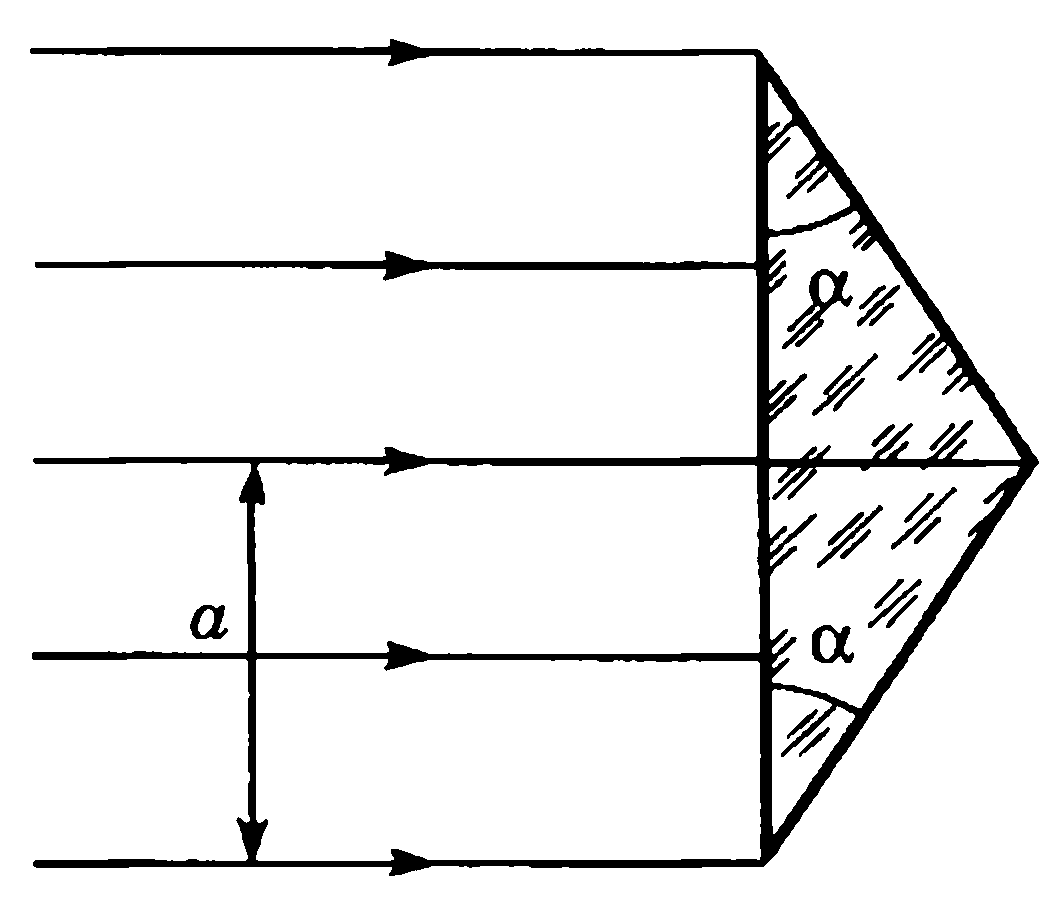
\includegraphics[width=0.4\columnwidth]{figures/4_11}
           \caption{.}
           \label{fig:4_11}
        \end{figure}

\section{ლინზები}

\textbf{4.48} სურათზე \ref{fig:4_48} ნაჩვენებია სინათლის წერტილოვანი წყარო $S$, მისი გამოსახულება $S_1$ მიღებული ლინზის საშუალებით და $OO_1$ ლინზის მთავარი ოპტიკური ღერძი. აგების მეშვეობით განსაზღვრეთ ლინზის მდებარეობა და იპოვეთ მისი ფოკუსები. ნამდვილია თუ წარმოსახვითი მიღებული გამოსახულება?
		\begin{figure}[h]
		   \centering
           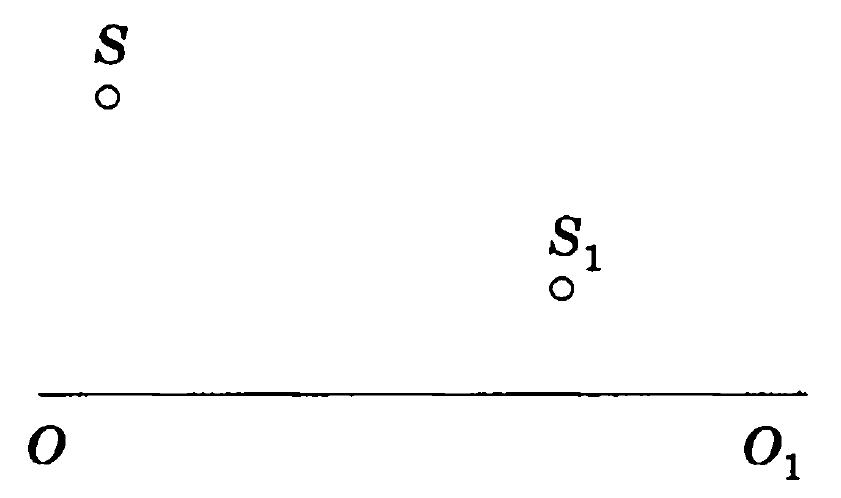
\includegraphics[width=0.4\columnwidth]{figures/4_48}
           \caption{.}
           \label{fig:4_48}
        \end{figure}

\textbf{4.49} სურათ \ref{fig:4_49}-ზე მოცემულია $ABC$ სხივის სვლა გამბნევ ლინზაში. აგების მეშვეობით განსაზღვრეთ ლინზის ფოკუსები. 
		\begin{figure}[h]
		   \centering
           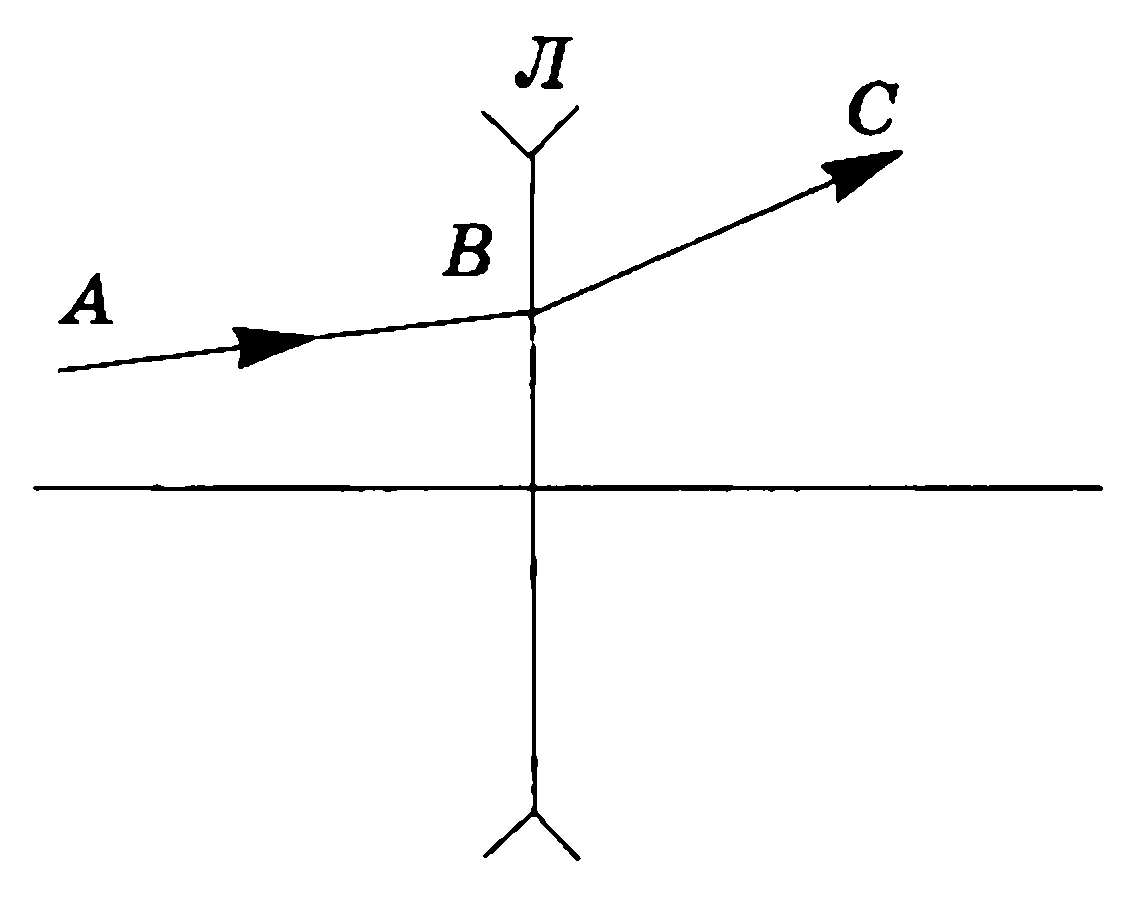
\includegraphics[width=0.4\columnwidth]{figures/4_49}
           \caption{.}
           \label{fig:4_49}
        \end{figure}

\textbf{4.52} რა $d$ მანძილზე უნდა მოვათავსოთ საგანი შემკრები ლინზიდან, რომ მანძილი ამ საგანს და მის ნამდვილ გამოსახულებას შორის იყოს უმცირესი? ლინზის ფოკუსური მანძილი ტოლია $F$.

\textbf{4.55} მანძილი საგანს და ლინზით მიღებულ, მის პირდაპირ გამოსახულებას შორის ტოლია $l = 5$ სმ, გამოსახულება გადიდებულია $\beta = 0.5$-ით. განსაზღვრეთ ლინზის ფოკუსური მანძილი.

\textbf{4.56} ეკრანზე ლინზის მეშვეობით მიღებულია გამოსახულება $\beta_1 = 2$ გადიდებით. როგორი იქნება გადიდება, თუ მანძილს საგანსა და ეკრანს შორის გავადიდებთ 1.6-ჯერ?

\textbf{4.57} ლინზა ფოკუსური მანძილით, $F = 12$ სმ ქმნის ეკრანზე საგნის გამოსახულებას $\beta_1 = 9$ გადიდებით. მეორე ლინზა იგივე მანძილზე საგანსა და ეკრანს შორის იძლევა $\beta_2 = 3$-ით გადიდებულ გამოსახულებას. იპოვეთ მეორე ლინზის ფოკუსური მანძილი.

\textbf{4.58} მიმართული სინათლის კონის მისაღები ფანარი შედგება, სინათლის წერტილოვანი წყაროსა და და ლინზისაგან დიამეტრით $D = 6$ სმ და ფოკუსური მანძილით $f = 15$  სმ. რა მანძილით უნდა იყოს დაშორებული ლინზიდან წყარო, რომ ლინზაში გამავალი სხივები ქმნიდნენ ეკრანზე $d = 4$ სმ-იან სინათლის ლაქას? ლინზიდან ეკრანამდე მანძილია $L = 100$ სმ.

\textbf{4.59} საგანი და მისი პირდაპირი გამოსახულება სიმეტრიულადაა განლაგებული ლინზისა ფოკუსის მიმართ. საგნიდან ლინზის ფოკუსამდე მანძილია $l = 4$ სმ. იპოვეთ ლინზის ფოკუსური მანძილი.

\textbf{4.60} შემკრები ლინზის უკანა ფოკუსსა და გამოსახულებას შორის მანძილი 9-ჯერ მეტია ვიდრე მანძილი წინა ფოკუსსა და ლინზას შორის. იპოვეთ ლინზის გამადიდებლობა.
       
\textbf{4.61} ლინზის მეშვეობით იღებენ საგნის ნამდვილ $\beta = 1.5$-ჯერ გადიდებულ გამოსახულებას. შემდეგ ლინზას გადააადგილებენ $l = 12$ სმ მანძილით და იღებენ იგივე ზომის წარმოსახვით გამოსახულებას. განსაზღვრეთ ლინზის ფოკუსური მანძილი.

\textbf{4.63} ცდის საშუალებით განსაზღვრეს დამოკიდებულება $\beta$ გამადიდებლობასა და ლინზასა და ეკრანს შორის შორის $b$ მანძილზე \ref{fig:4_63}. განსაზღვრეთ ლინზის ფოკუსური მანძილი.
		\begin{figure}[h]
		   \centering
           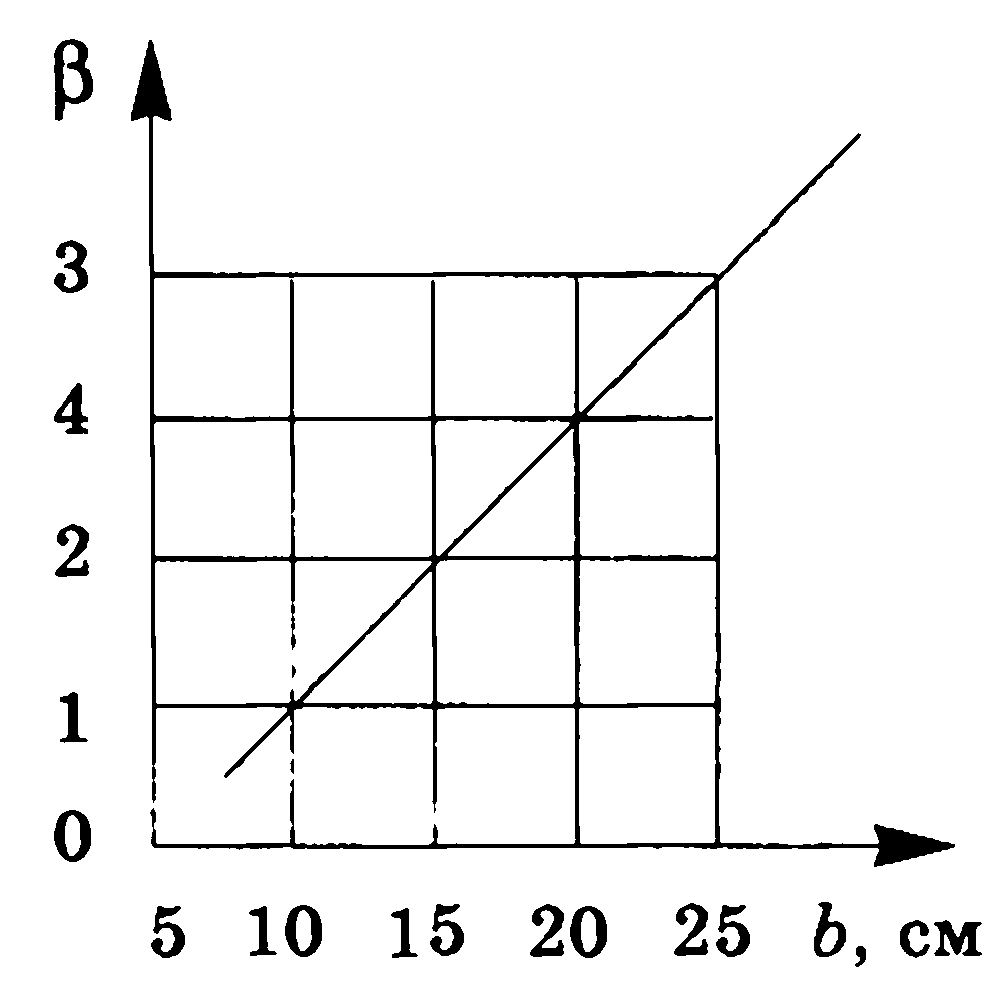
\includegraphics[width=0.4\columnwidth]{figures/4_63}
           \caption{.}
           \label{fig:4_63}
        \end{figure}

\textbf{4.64} შემკრები ლინზიდან

\textbf{4.75} ორი შემკრები ლინზა ფოკუსური მანძილებით $F_1$ და $F_2$ მოთავსებულია ერთ ღერძზე. ამ სისტემების მეშვეობით იღებენ საგნის გამოსახულებას, აღმონჩდა რომ მიღებული გამოსახულების ზომა არაა დამოკიდებული ლინზათა სისტემასა და საგანს შორის მანძილზე. იპოვეთ ლინზათა შორის მანძილი. 
\end{document}